\section{Method}
\label{sec:locvqallm_method}


In general, a \gls{vqa} model with parameters $\thetabf$ generates an answer $\hat{a}$ when given an input image $\x \in \real^{H\times W\times C}$ and a related question represented as a sequence of words, $\q$. %Here, $H$, $W$, and $C$ denote the height, width, and channels of the image, respectively. 
In its most general form, this process can be described as a function $\Psi_{\text{VQA}}$, parameterized by $\thetabf$, that is applied on the image-question pair,
\begin{equation}
    \hat{a} = \Psi_{\text{VQA}} (\x, \q; \thetabf).
\end{equation}
Traditionally, this model's output is a distribution over a set of $N$ candidate answers $\{a_1, a_2, ..., a_N\}$ set beforehand. 

In this work, however, we choose the answer of the \gls{vqa} to be generated by an \gls{llm} in an auto-regressive manner until the end-of-sentence (EOS) token is produced. To make the \gls{llm} multimodal, we adopt the widely used approach of projecting visual embeddings onto the input space of the \gls{llm}~\cite{liu2023visual,tsimpoukelli2021multimodal,wang2023r2gengpt} and 
express this as 
\begin{equation}
    \hat{a} = \Psi_{\text{LLM}} (\Psi_{\text{Vis}} (\x, \thetabf_{\text{Vis}})\W^\text{proj}, \q; \thetabf_{\text{LLM}}),
\end{equation}
\noindent
where $\Psi_{\text{Vis}}$ refers to the visual encoder with parameters $\thetabf_{\text{Vis}}$, and $\W^\text{proj}$ denotes the learnable parameters of the projection layer. Although not explicitly formalized, it is implied that the answer is generated in an auto-regressive fashion, meaning that the next word in the answer depends on the previously predicted words.

To expand the model's capability to handle localized questions, we propose here a dedicated targeted visual prompt that allows two perspectives of the image to be encoded: one containing only the region of the image and the other containing the region in context. 

The targeted visual prompt consists of five components: (1) comprises model instruction, denoted as $\w_{\text{instr}}$; (2) the visual context represented by the image with the region drawn on it, $\x_r$; (3) $\w_\text{det}$ contains a textual prefix for the region; (4) the cropped region $\rbf$; and (5) $\w_q$ includes the question $\q$. Text-containing parts of the prompt undergo tokenization and embedding, while the visual components are processed by a visual encoder and then projected into the input space of the \gls{llm}. Subsequently, the results are concatenated and processed by the \gls{llm}, resulting in the generation of an answer. To handle global questions, the entire image is assigned to $\rbf$. We illustrate our model in Fig.~\ref{fig:method} and summarize the computation of the answer as,
\begin{equation}
    \hat{a} = \Psi_{\text{LLM}} (\w_{\text{instr}}, \Psi_{\text{Vis}} (\x_r, \thetabf_{\text{Vis}})\W^\text{proj}, \w_\text{det}, \Psi_{\text{Vis}} (\rbf, \thetabf_{\text{Vis}})\W^\text{proj}, \w_q; \thetabf_{\text{LLM}}),
\end{equation}

\begin{figure}[!t]
\begin{center}
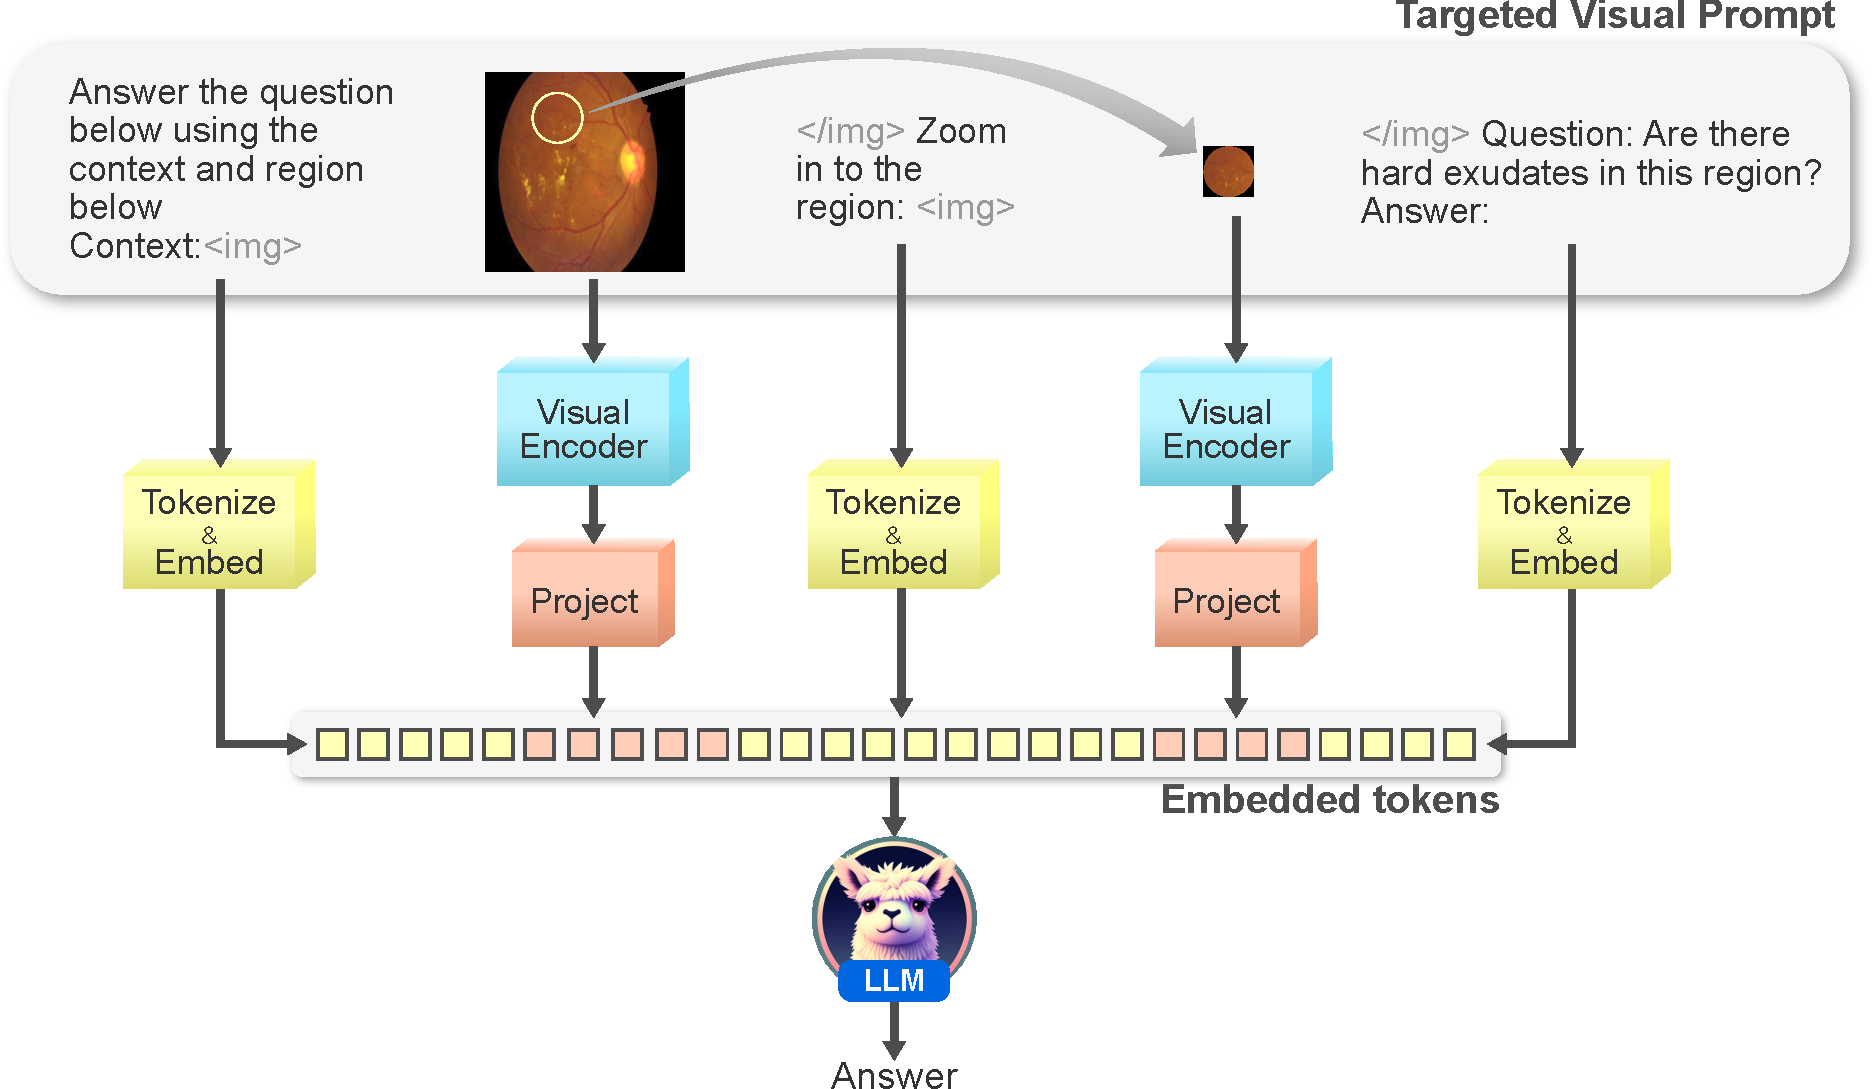
\includegraphics[width=\textwidth]{Figures/Part1_LocVQA/02_llm/method.pdf}
\caption{Our customized targeted visual prompt is created by providing the model with the region in context, as well as an isolated version of the region. Visual tokens are projected to the input space of the LLM and concatenated with the instruction tokens.}
\label{fig:method}
\end{center}
\end{figure}

\textbf{Training. } As in~\cite{wang2023r2gengpt}, our model is trained using the original auto-regressive training loss of the \gls{llm}. The loss function is the standard negative log-likelihood accumulated over all time steps for predicting the correct next token. For a ground truth answer of length $T$, this loss is expressed as,
\begin{equation}
    \mathcal{L}(\thetabf) = - \sum_{t=1}^T \log p_\theta(a^t | \x, \w, a^{1:t-1}; \thetabf),
\end{equation}
\noindent
where $\x$ and $\w$ denote the visual and textual elements, respectively, and $\mathbf{a} = \{a_1, a_2, ..., a_T\}$ is the ground truth answer.